\documentclass[10pt,a4paper]{article}
\usepackage[utf8]{inputenc}
\usepackage{amsmath}
\usepackage{amsfonts}
\usepackage{amssymb}
\usepackage{graphicx}
\usepackage[english]{babel}

\author{Daniel Underwood}
\title{Polycyclic Aromatic Hydrocarbons Modelled as Particle in Box to Determine Length}

\begin{document}
\maketitle

\section*{Introduction}

The purpose of this experiment is to determine a theoretical length of the polycyclic aromatic hydrocarbon compounds naphthalene, anthracene, and tetracene by modelling the molecules as a particle two-dimensional infinite square box and compare the theoretical values of this model with experimentally obtained values.

These compounds may be modelled in this way since the benzene rings within the molecule have de-localized electrons that are free to move throughout the molecule as long as they remain within in the plane of the molecule, resulting in a simplification to a two-dimensional model. While these electrons are free to move throughout the molecule, they are restricted from moving past the end of the molecule. While there is an exponential probability for the electrons to go beyond what is the length of the molecule, the simplification of making that region forbidden is a good approximation. Forbidding these electrons in these regions results in an infinite potential at the ends, which results in a 2D infinite square well.

\section*{Methods}

The experimental values are obtained by obtaining the energy gap between the highest occupied molecular orbital (HOMO) and lowest unoccupied molecular orbital (LUMO) levels of the molecules.

The transition between these levels is determined by taking an absorption spectrum of a solution of the compounds. The wavelength with the maximum absorption coefficient is the HOMO/LUMO transition. The absorption spectrum only determines the wavelength and thus energy gap of the transition, and we must know the HOMO/LUMO levels. The actual HOMO/LUMO levels are determined by the fact that each C=C results in 2 $\pi$-electrons. The HOMO level may simply be determined by the number of C=C bonds in the molecule. This results in naphthalene, anthracene, and tetracene  respectively having HOMO levels of 5, 7, and 9 with LUMO levels of one more, or 6, 8, and 10.

The absorption spectra were obtained with an Ocean Optics USB4000 spectrometer. The solutions of naphthalene, anthracene, and tetracene were all $100 \mu \rm{M}$ solutions in 1-Octanol. A sample of 1-Octanol was used for the spectrometer's baseline to remove the background spectrum of the solute.

The theoretical length of the molecules were determined with geometry and the bond lengths of 1.40\AA\, for a C--C bond and 1.33\AA \,for a C=C bond. Theoretical lengths for naphthalene, anthracene, and tetracene were found to be 4.84\AA, 7.26\AA, and 9.68\AA, respectively.

\begin{equation}
E = \frac{hc}{\lambda}
\end{equation}

Using Equation (1), the energy gap between the HOMO and LUMO levels is able to be determined using the wavelength of the highest absorption for $\lambda$. This resulted in energy gaps of 4.32eV, 4.88eV, and 4.32eV energy gaps for naphthalene, anthracene, and tetracene, respectively. Using this energy gap with Equation (2) yields the length of the molecule as represented by the infinite square well.

\begin{equation}
L = \frac{hn}{2} \sqrt{\frac{1}{2 m_e E}}
\end{equation}

\section*{Results}

The spectroscopic data collected is plotted for all of the molecules in Figure 1. A notable feature of this data is the double peak for naphthalene. The highest absorption in the collected data was located at $287.32\rm{nm}$, so that value is used for the determination of the length of the molecule.

\begin{figure}[h]
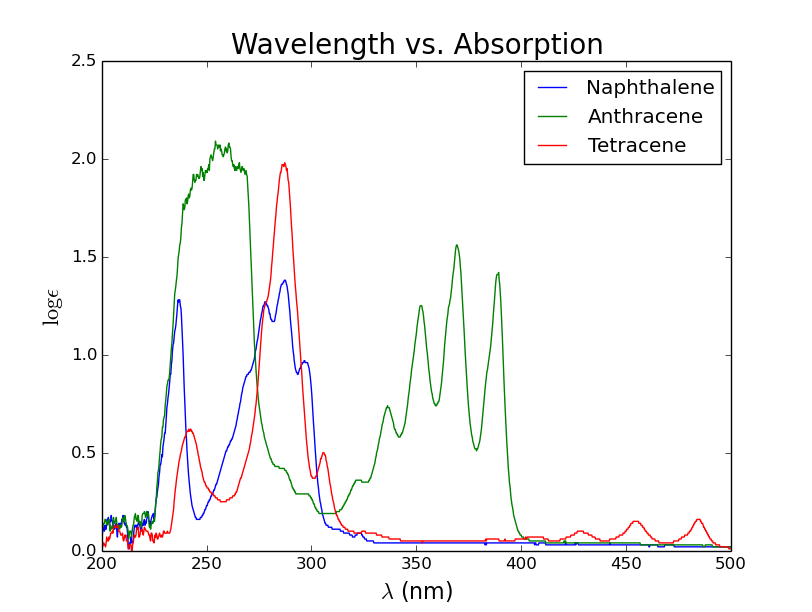
\includegraphics[width=\linewidth]{plot.png}
\caption{Wavelength vs. Absorption of Molecules}
\end{figure}

Table 1 contains the values found experimentally along with their theoretical counterpart and the percent difference of each.

\begin{table}[h]
\begin{tabular}{cccc}
Molecule & Experimental Length (\AA) & Theoretical Length (\AA) & \% Difference \\
\hline
Naphthalene & 5.91 & 4.81 & 22.87 \\
Anthracene & 7.41 & 7.26 & 2.07\\
Tetracene & 9.85 & 9.68 &  1.76

\end{tabular}
\caption{Results}
\end{table}

\section*{Discussion}

The largest discrepancy with the experiment is the large difference between experimental and theoretical values of the naphthalene sample. One reasonable explanation for this is the double peak. If the first peak were used, the experimental length would likely be much closer to the theoretical value.

An obvious feature of the results is the fact that the error goes down as the molecule gets larger. A plausible explanation for this is that the limit $N \to \infty$, where $N$ is the number of benzene molecules in the chain, leads to the ideal case of a pure sine wave representing the electrons' locations. As the molecule gets smaller, the potential at the ends is lower and there is a slower exponential decay, resulting in a higher probability of the electrons being farther from the end of the molecule.

\section*{Conclusion}

In conclusion, while this model is not entirely accurate, it makes an excellent approximation for many cases. If a model that also included exponential terms at the ends of the molecules were used, it would have likely reduced the discrepancy between the theoretical and experimental values.
\end{document}